%\chapter{Implementation}\label{s:implementation}
%\graphicspath{ {./images/} }
%\begin{figure}[t]
%\centering
%\caption{Zoomed in on QAS of ASR-1}
%\label{fig:ASR2}
%\end{figure}
%\includegraphics[width=12cm]{Decomposition of ASR and QAS_zoomed in on %ASR-1 and ASR-2_v2.jpg}\\
\chapter{Implementation}\label{s:Implementation}
Research question 3 focuses on patterns and tactics, in context of software architecture. Bass \etal \cite{Bass2015SoftwareAI} describes architectural patters as "Compositions of architectural elements and provide packaged strategies for solving some of the problems facing a system." This section contains examples of processes represented by views and contain patterns and tactics. Focusing on the quality attribute 'Confidentiality', which is the quality attribute that could mitigate the operational problems in section \ref{OP} The pattern of 'Zero-knowledge proof' and tactics of 'Data minimization' and 'Pseudonymization' mentioned by consulted experts as possible techniques to apply. By depicting different types of views on example processes, the examples are presented as possible basis for practical use. The tactics of Authentication' and 'Encryption' are more basic building blocks already applied and therefore explained more briefly.

Section \ref{QI} discusses the quantified problem and argues logical reasoning will define how a solution could mitigate the operational problem mentioned in section \ref{OP}
\section{Pattern - Zero-knowledge proof}
By definition of Goldwasser \etal \cite{Goldwasser} "A zero-knowledge proof (ZKP) makes it possible to prove a statement is true while preserving confidentiality of secret information". 
Xiaohui Yang and Wenjie Li \cite{YANG2020102050} state "Zero-knowledge proof (ZKP) is a cryptography technique, which means that the prover can convince the verifier that a certain statement is correct without providing the verifier with any additional information or leaking any information about the witness." Figure \ref{fig:ZKP_usecase} presents a schema on how this principle works. Figure \ref{fig:QAS01} presents two example Quality Attribute Scenarios (QAS) which describe desired system behaviour. The ZKProof Community reference \cite{2019:zkproof:community-reference-0.2} of Bennarroch \etal is intended to provide a reference for development of zero-knowledge proof by contribution of world-renowned cryptographers, practitioners and industry leaders.
Reasoning why this methodology or pattern is a solution for the operational problem in section \ref{OP} is if there is no identity data to be shared or replicated, there will be no profiling or unauthorized correlation of identity data can be done. Without identity data it's not possible to commit identity fraud.

\subsection{Chain of use-cases described}
\graphicspath{ {./images/} }
\begin{figure}
\centering
\label{fig:ZKP_usecase}
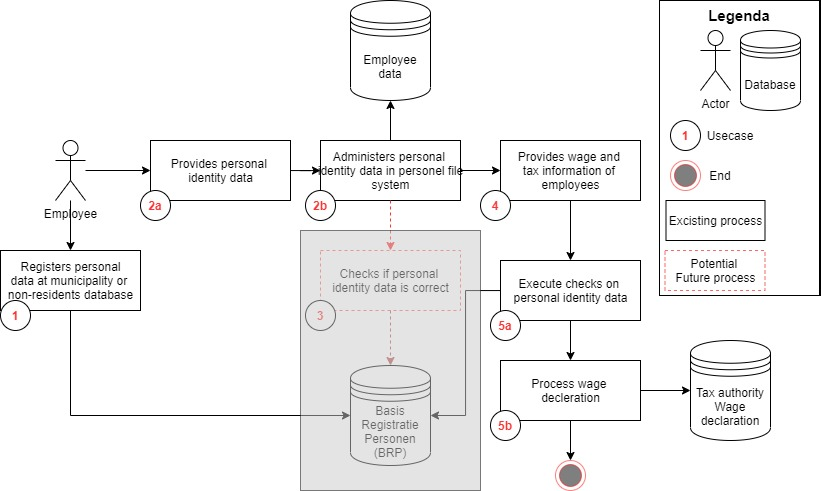
\includegraphics[width=10cm]{Usecase for zkp.jpg}\\
\caption{Scenarios - set of use-cases on one of ZKP could be applied}
\end{figure}

\graphicspath{ {./images/} }
\begin{figure}
\centering
\label{fig:QAS01}
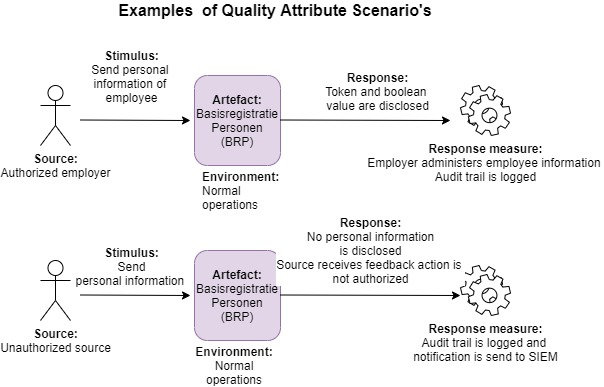
\includegraphics[width=7cm]{QAS-01 ZKP.jpg}\\
\caption{Example of Quality attribute scenario's}
\end{figure}


Zero-knowledge proof itself is a methodology which translates in a variety of technical implementation possibilities. Suitability needs to be assessed per use-case, therefore this research contains an example with high-level scenarios and use-cases depicted in figure \ref{fig:ZKP_usecase}.

This use-case contains three acting parties, namely the employee, employer and tax authorities (Belastingdienst).
Firstly a citizen registers finishes it's registration of personal data at a municipality or non-residents database desk. After this process is finished the citizen receives a BSN, which serves as a UIN throughout all government administrations. The citizen starts working at an employer, fills in his personal information for the wage declaration, including the BSN (2a). The employer is responsible to administer personal information of its employee (2b) and administer and transfer wage declaration to the tax authorities (4). Based on the BSN in the wage declaration, the tax authority checks the personal identity data (5a). \par
In the happy flow, all information off the employee is correct and wage declaration is processed correctly (5b). However, there are practical exceptions, where an employer administers an incorrect BSN or the set of personal information does not match that BSN. In this case, the wage declaration is processed incorrectly. Impact can be another citizen, with the wrongly entered BSN, being taxed for the wage of another citizen. Correcting this mistakes are costly for the government and intense for a citizen who could be negatively impacted because of a higher wage.

\subsection{Use-case 3: application of zero-knowledge proof}
A possible solution would be to let the employer check the correctness of personal information when hiring a citizen. Section \ref{BRP} describes the BRP as the central database of personal identity data of citizens and could be used for this purpose. However, pushing information from the BRP to an employer is not legally allowed. One of the risks could be not acting in good faith which could result in scraping the database to commit fraud or unauthorized usage of personal data mentioned in section \ref{OP}. Zero-knowledge proof could be a pattern to resolve this problem by providing a check if the data the employer receives from an employee matches with a person in the BRP. Ideally, a Zero-knowledge proof will result in not saving personal information in an employer database. However, if this is mandatory by law it needs to been done or law needs to be changed.
\clearpage

\section{Tactics - Quality attribute 'Confidentiality'}
\graphicspath{ {./images/} }
\begin{figure}
\centering
\label{fig:Tactics}
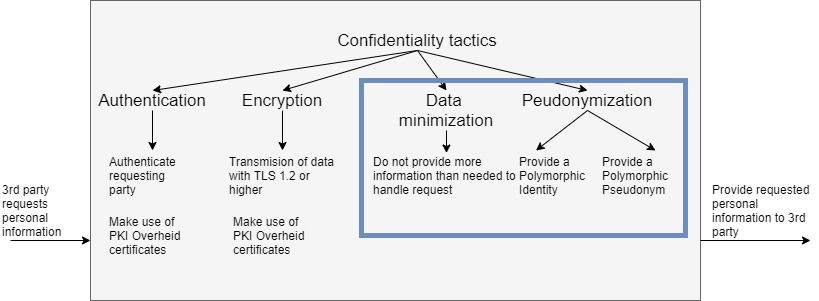
\includegraphics[width=14cm]{Tactics.jpg}\\
\caption{Confidentiality tactics - next section handles examples in blue frame}
\end{figure}

\subsection{Data minimization}
Demanding parties of personal information who are legally permitted to consult the BRP need to search for a person of interest residing on an address. In this case, it can be assumed the personal information has to be shown of only this person of interest. A query which is too broad could give back results of multiple persons. Which could be considered a breach of privacy of those persons. Figure \ref{fig:Adhoc} illustrates a logical view on how a tactic of data minimization could be applied. Firstly, a possible scope of addresses is queried on the Basisadministratie Gebouwen (BAG) \cite{BAG}. The BAG contains almost all addresses within the Dutch territory. Secondly, the correct address is shown and can be selected from this query. If query is a specific statement and returns one result, this result can be selected automatically to support usability. Thirdly, based on the unique address ID from the BAG a list of resident is shown with a minimal set of information to assess if the results contain the person of interest.    
\graphicspath{ {./images/} }
\begin{figure}
\centering
\label{fig:Adhoc}
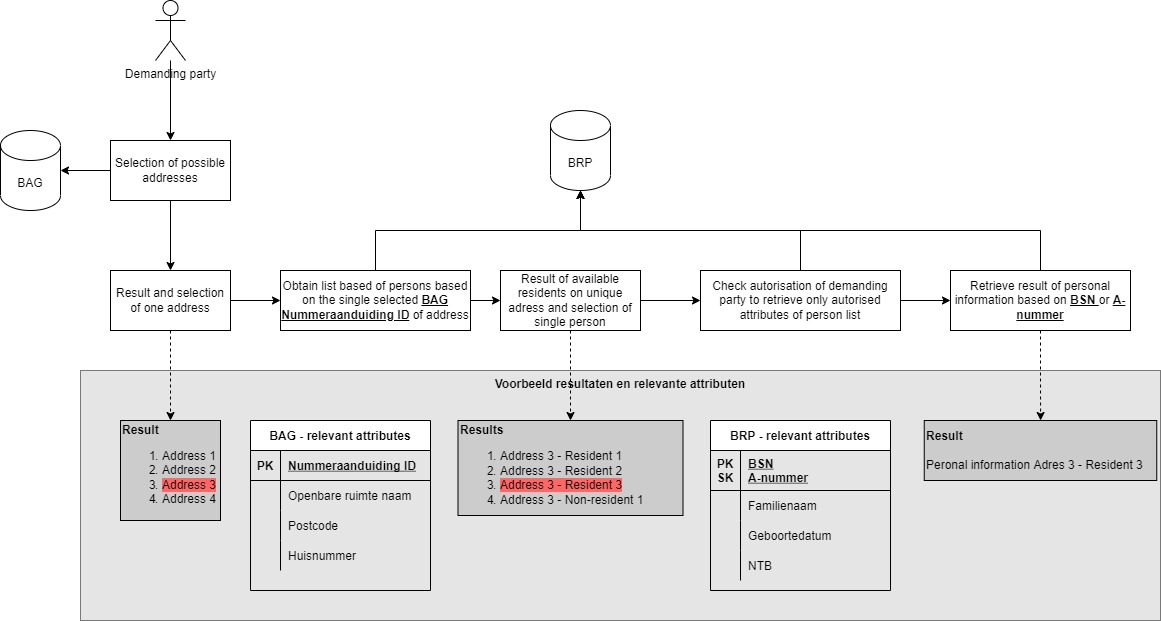
\includegraphics[width=14cm]{Ad-hoc adresvraag dataminimalisatie-EN.jpg}\\
\caption{Logical view - example of data minimization in a process}
\end{figure}

\subsection{Pseudonymization - Polymorphic Identity or Polymorphic Pseudonym}
When it's mandatory to share personal information, because it's for example mandatory by law, it's possible to provide this information as a pseudonym. GDPR \cite{GDPR} defines this method as a possibility to mitigate unwanted disclosure of personal information. 
This technique is already implemented and proven it can work by Erik Verheul \cite{VerheuleID}.

\subsection{Authentication}
A commonly used method for authentication purposes is usage of a certificate. For parties who communicate with on or on behalf of the Dutch government the government issues PKIoverheid (PKIO) certificates. These certificates are used for Authentication, Electronic signatures and encryption. \cite{Logius_PKIO}

\subsection{Encryption - Transfer of data is encrypted with TLS 1.2 or higher}
A broadly implemented standard. The Dutch government has a reference architecture NORA (Nederlandse Overheid Referentie Architecture) \cite{NORA} which states this standard needs to be applied or otherwise explained why it has not been implemented \cite{NORA_PasToeOfLegUit}. On the part of TLS its clear version 1.2 or higher is accepted, but version 1.3 is preferred \cite{NORA_TLS}. 

\section{Trade-offs and concerns}
\todo{Scrapbook, needs refinement}


\begin{tblr}{
 hlines = {white},
 vlines = {white},
 cell{2,3,4,5,6}{1} = {red7}
}
  & Trade-off & Concern & Threats and risk \\
 Maturity & 1 & C-xx, C-xx, C-xx & 3 \\
 Authenticity & 1 & C-xx, C-xx, C-xx & 3 \\
 Accountability & 1 & C-xx, C-xx, C-xx & 3 \\
\end{tblr}

Trade-off snelheid/efficientie. Depends on choosen methodology and algoritm. It's needed to address the needed calculation power (and assumed costs) when selecting algoritms 
\todo{Better describe and support these trade-offs and concerns}



%%% Local Variables:
%%% mode: latex
%%% TeX-master: "../thesis"
%%% End:
